%
% rossby.tex
%
% (c) 2018 Prof Dr Andreas Müller, Hochschule Rapperswil
%

\section{Rossby-Wellen\label{section:elnino:rossby}}
In der Untersuchung der Kelvin-Wellen haben wir angenommen, dass die
Geschwindigkeit $v$ entlang der Längenkreise verschwindet.
Die Strömung wird im allgemeinen nicht parallel zum Äquator sein.
Trotzdem beobachten wir zum Beispiel, dass die Westwindströmung 
zwischen verschiedenen geographischen Breiten mäandriert.
Woher kommt diese Wellenbewegung?

\subsection{Zirkulation\label{subsection:rossby:zirkulation}}
Aus der Diskussion der globalen Zirkulation wissen wir, dass die
Strömung in Äquatornähe dominiert wird durch eine mittlere Strömung
konstante Strömung mit Geschwindigkeit $U$ in Ost-West-Richtung.
Wir suchen daher eine Beschreibung der Abweichungen von dieser
mittleren Strömung.
Unter Verwendung der gleichen Notation wie im
Abschnitt~\ref{section:elnino:kelvin} schreiben wir daher
\[
u=U+u',\qquad v=U+v'\qquad\text{mit $u,v\ll U$}.
\]


Wir nehmen im folgenden wieder an, dass die Strömung quellenfrei ist.
Dann lässt sich wie früher gezeigt, dass die Strömung mit einer
Strömungsfunktion $\psi$ als
\[
u=-\frac{\partial \psi}{\partial y},\qquad
v=\frac{\partial\psi}{\partial x}
\]
beschrieben werden kann.

Die Drehimpulsdichte in der Strömung ist gegeben durch die Zirkulation
\[
\zeta
=
\frac{\partial v}{\partial x} - \frac{\partial u}{\partial y}
=
\Delta \psi.
\]
Da der Drehimpuls erhalten ist, muss die Zirkulation in einem
Luftpacket abnehmen, wenn es sich auf der Nordhalbkubel nach Norden
bewegt.
Die Quelle dieser Zirkulationsänderung ist die Erddrehung und damit
die Corioliskraft $f$ und der mathematische Ausdruck der Drehimpulserhaltung
ist die Erhaltung der Grösse $\zeta+f$.

\subsection{Bewegungsgleichung\label{subsection:rossby:bewegungsgleichung}}
Die Grösse $\zeta+f$ ist erhalten, ihre zeitliche Ableitung
\[
\frac{d(\zeta f)}{dt}=0
\]
verschwindet also.
$f$ hängt nur von $y$ ab, aber die Funktion $\zeta$ hängt von $t$,
$x$ und $y$ ab.
Wir berechnen die Ableitung mit Hilfe der Kettenregel:
\begin{align*}
0
=
\frac{d(\zeta+f)}{dt}
&=
\frac{\partial\zeta}{\partial t}
+
\frac{\partial\zeta}{\partial x}\cdot \frac{dx}{dt}
+
\frac{\partial(\zeta+f)}{\partial y}\cdot\frac{dy}{dt}
\\
&\simeq
\frac{\partial\zeta}{\partial t}
+
(U+u)\frac{\partial\zeta}{\partial x}
+
v\biggl(\frac{\partial\zeta}{\partial y} + \frac{\partial f}{\partial y}\biggr).
\end{align*}
Da $u\ll U$ ist, kännen wir in erster Näherung $u$ im zweiten Term 
vernachlässigen.
Und da $\partial\zeta/\partial y$ ebenfalls sehr klein ist, können
wir dies im letzten Term im Vergleich zu $\partial f/\partial y$
vernachlässigen.
Schliesslich können wir wie in Abschnitt~\ref{section:elnino:kelvin}
die $\beta$-Ebenen-Approximation verwenden, und $\partial f/\partial y$
durch $\beta$ ersetzen.
Schliesslich können wir wieder $v=\partial\psi/\partial x$ ersetzen.
Wir erhalten so
\[
0
=
\frac{\partial\zeta}{\partial t}
+
U\frac{\partial\zeta}{\partial x}
+
\beta\frac{\partial\psi}{\partial x}
\]
als Bewegungsgleichung.

Indem wir $\zeta=\Delta \psi$ schreiben, erhalten wir so die 
Bewegungsgleichung
\begin{equation}
\frac{\partial\Delta\psi}{\partial t}
+
U\frac{\partial\Delta\psi}{\partial x}
+
\beta\frac{\partial\psi}{\partial x}
=
0.
\label{rossby:gleichung}
\end{equation}


\subsection{Wellenlösungen\label{subsection:rossby:loesungen}}
Gesucht sind Lösungen der Gleichung~\eqref{rossby:gleichung}
in Form kleiner Abweichungen.
Wir erwarten Wellenlösungen und schreiben sie daher in der Form
\begin{equation}
\psi_{kl}(t,x,y)
=
\sin(kx+ly-\omega t).
\label{rossby:ebenewelle}
\end{equation}
Die Ableitungen, die wir für die Bewegungsgleichung
\eqref{rossby:gleichung} benötigen, sind
\begin{align*}
\frac{\partial}{\partial t} \psi_{kl}(t,x,y)
&=
-\omega \cos(kx+ly-\omega t) = -\omega\psi_{kl}(t,x,y),
\\
\frac{\partial}{\partial x} \psi_{kl}(t,x,y)
&=
k
\cos(kx+ly-\omega t) = k \psi_{kl}(t,x,y),
\\
\Delta\psi_{kl}
&=
-(k^2+l^2)\cos(kx+ly-\omega t)=-(k^2+l^2)\psi_{kl}(t,x,y).
\end{align*}
Setzen wir dies in die Differentialgleichung ein, erhalten wir 
\begin{align*}
0
&=
\omega(k^2+l^2)\psi_{kl}(t,x,y)
-
Uk(k^2+l^2)\psi_{kl}(t,x,y)
+
\beta k\psi_{kl}(t,x,y)
\\
&=
\bigl((\omega-Uk)(k^2+l^2)+\beta k\bigr)\psi_{kl}(t,x,y)
\end{align*}
Für eine Lösung muss also die Dispersionsrelation
\[
(\omega -Uk)(k^2+l^2) +\beta k=0
\]
gelten.
Aufgeläst nach $\omega$ ist dies
\begin{align}
\omega(k^2+l^2)
&=
Uk(k^2+l^2) -\beta k
\notag
\\
\Rightarrow\qquad
\omega
&=
Uk
-
\frac{\beta k}{k^2+l^2}.
\label{rossby:dispersion}
\end{align}
Eine Wellenlösung mit Wellenzahlen $k$ und $l$ hat daher 
die Ausbreitungsgeschwindigkeit 
\begin{equation}
c=\frac{\omega}{k} = U-\beta\frac{1}{k^2+l^2}
\label{rossby:phasengeschwindigkeit}
\end{equation}
entlang der $x$-Koordinate.
Da der Nenner immer positiv ist, ist $c$ kleiner als $U$, solche
Wellen können sich immer nur in West-Ost-Richtung ausbreiten.

\subsection{Gruppengeschwindigkeit}
Die Phasengeschwindigkeit~\eqref{rossby:phasengeschwindigkeit}
hilft uns nicht, die Dynamik des El Niño zu verstehen, da wir dazu
den Transport von Energie verstehen müssen.
Die ebenen Wellen der Form~\eqref{rossby:ebenewelle} beschreiben eine Welle
die überall die gleiche Amplitude hat, es findet also eigentlich gar
kein Energietransport statt.
Im Beispiel des ``Wasserberges'' in der Untersuchung zu den Kelvin-Wellen
wird potentielle Energie dadurch transportiert, dass das Wasser des Berges
abfliesst.
Wir müssen daher erst einen ``Wasserberg'' als Überlagerung von 
ebenen Wellen formulieren und dann die zeitliche Entwicklung dieser
Überlagerung studieren.

\subsubsection{Überlagerungen}
Wir gehen daher von einer eindimensionalen Situation aus und studieren
eine Überlagerung $u(x,t)$ von Wellen der Form $\cos(kx-\omega(k) t)$
mit verschiedenen Wellenzahlen $k$.
Mit der Wellenzahlabhängigen Amplitude $\hat f(k)$ lässt sich die
Überlagurung als
\begin{equation}
u(x,t)
=
\int_{-\infty}^\infty \hat f(k)\,\cos(kx-\omega(k)t)\,dk
\label{rossby:reelleueberlagerung}
\end{equation}
schreiben.
Die Bewegung eines solchen Wellenpaketes kann man zum Beispiel
dadurch studieren, dass man die Bewegung des Maximums dieses 
Wellenpaketes verfolgt.

Die Darstellung~\eqref{rossby:reelleueberlagerung} ist für diese
Untersuchung sehr unhandlich, die Rechnung sind sehr umständlich.
Wir schreiben die Wellen daher als Realteil einer komplexen
Welle $e^{i(kx-\omega(k)t}$, also
\begin{equation}
u(x,t)
=
\operatorname{Re}
\int_{-\infty}^\infty \hat f(k)\,e^{i(kx-\omega(k)t)}\,dk.
\label{rossby:komplexeueberlagerung}
\end{equation}

\subsubsection{Wellenpakete}
\begin{figure}
%\def\deltak{0.6}
%\def\knull{12}
%\def\ampli{0.25}
%\begin{tikzpicture}[>=latex,thick]
%\begin{scope}[xshift=-6cm]
%\draw[->] (-0.1,0)--(5.1,0) coordinate[label={$k$}];
%\draw[->] (0,-0.1)--(0,2.3) coordinate[label={right:$\hat f(k)$}];
%\draw[color=red,line width=1.4pt] (-0.1,0)--({3-0.2},0);
%\draw[color=red,line width=1.4pt] ({3+0.2},0)--(5.1,0);
%\draw[color=red,line width=1.4pt] ({3-0.2},2)--({3+0.2},2);
%\draw[color=red,line width=0.1pt] ({3-0.2},0)--({3-0.2},2);
%\draw[color=red,line width=0.1pt] ({3+0.2},0)--({3+0.2},2);
%\draw[line width=0.1pt] (0,2)--(5,2);
%\draw (-0.1,2)--(0.1,2);
%\draw (3,-0.1)--(3,0.1);
%\draw ({3-0.2},-0.1)--({3-0.2},0.1);
%\draw ({3+0.2},-0.1)--({3+0.2},0.1);
%\node at (3,0) [below] {$k_0$};
%\node at ({3-0.2},0) [above left] {$k_0-\Delta k$};
%\node at ({3+0.2},0) [above right] {$k_0+\Delta k$};
%\end{scope}
%\begin{scope}[xshift=4cm,yshift=1cm]
%\draw[->] (-3.1,0)--(3.1,0) coordinate[label={$x$}];
%\draw[->] (-3,-1.1)--(-3,1.3) coordinate[label={right:$u(x,t)$}];
%\draw[color=red] plot[domain=-3:3,samples=2400]
%	({\x},{\ampli*cos(360*\knull*\x)*sin(360*\deltak*\x)/\x});
%\draw[color=blue] plot[domain=-3:3,samples=400]
%	({\x},{\ampli*sin(360*\deltak*\x)/\x});
%\node at (0,-1) [below] {$x-ct$};
%\end{scope}
%\end{tikzpicture}
\centering
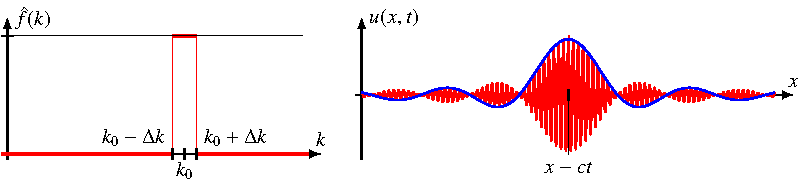
\includegraphics{chapters/7/wellenpaket.pdf}
\caption{Berechnung eines Wellenpaketes aus Wellen mit Wellenzahlen
zwischen $k_0-\Delta k$ und $k_0+\Delta k$.
\label{rossby:wellenpaket}}
\end{figure}
Wir betrachten ein Wellenpaket, welches als Überlagerung mit der
Funktion
\[
\hat f(k)
=
\begin{cases}
1&\qquad |k-k_0| < \Delta k\\
0&\qquad\text{sonst}
\end{cases}
\]
Die Überlagerung $u(x,t)$ gemäss~\eqref{rossby:komplexeueberlagerung}
kann man jetzt vereinfachen:
\[
u(x,t)
=
\int_{-\infty}^\infty \hat f(k)\,e^{i(kx-\omega(k)t)}\,dk
=
\int_{k_0-\Delta k}^{k_0+\Delta k} e^{i(kx-\omega(k)t)}\,dk,
\]
allerdings muss dazu $\omega(k)$ bekannt sein.

Falls $\omega(k)=ck$ gilt, falls also jede elementare Welle die gleiche
Ausbreitungsgeschwindigkeit $c$ hat, können wir $u(x,t)$ explizit
ausrechnen:
\begin{align*}
u(x,t)
&=
\operatorname{Re}
\int_{k_0-\Delta k}^{k_0+\Delta k}
e^{i(kx-\omega(k)t}\,dk
=
\operatorname{Re}
\int_{k_0-\Delta k}^{k_0+\Delta k}
e^{ik(x-ct)}\,dk
\\
&=
\operatorname{Re}
\biggl[
\frac{e^{ik(x-ct)}}{i(x-ct)}
\biggr]_{k_0-\Delta k}^{k_0+\Delta k}
=
\operatorname{Re}
\biggl(
\frac{e^{i(k_0+\Delta k)(x-ct)}}{i(x-ct)}
-
\frac{e^{i(k_0-\Delta k)(x-ct)}}{i(x-ct)}
\biggr)
\\
&=
\operatorname{Re}\frac{2}{x-ct}
e^{ik_0(x-ct)}\frac{e^{i\Delta k(x-ct)}-e^{i\Delta k(x-ct)}}{2i}
\\
&=
\operatorname{Re}\frac{2}{x-ct}
e^{ik_0(x-ct)}
\sin (\Delta k(x-ct))
=
2\cos k_0(x-ct) \frac{\sin \Delta k(x-ct)}{x-ct}
\end{align*}
Dies ist eine schnell schankende Funktion mit Wellenzahl $k_0$, rot
dargestellt in Abbildung~\ref{rossby:wellenpakt} rechts, moduliert
mit der langsam schwankenden Funktion $\sin\Delta k(x-ct)/(x-ct)$,
dargestellt in der selben Abbildung in blau.
Der Schwerpunkt des Paketes befindet sich bei der $x$-Koordinaten $x-ct$,
wandert also mit Geschwindigkeit $c$ nach rechts.

\subsubsection{Gruppengeschwindigkeit}
\index{Gruppengeschwindigkeit}%
Bisher haben wir angenommen, dass die Frequenz und die Wellenzahl proportional
sind, dass also $\omega(k)=ck$.
Die Untersuchungen zu den Rossby-Wellen hat gezeigt, dass dies nicht
zutreffen muss.
Wir müssen die Rechnung also mit einem Modell wiederholen, wo die
Frequenz $\omega(k)$ nicht einfach nur proportional zu $k$ ist.
Für kleines $\Delta k$ genügt eine lineare Approximation der
Abhängigkeit von $\omega(k)$ von $k$, wir setzen daher
\begin{equation}
\omega(k)
=
\omega(k_0) + (k-k_0)\omega_1
=
\omega_0 + (k-k_0)\omega_1
\qquad
\text{mit}
\quad
\omega_1 = \frac{d}{dk}\omega(k_0) = \omega'(k_0).
\end{equation}
Wir berechnen wieder $u(x,t)$ wie folgt:
\begin{align*}
u(x,t)
&=
\operatorname{Re}
\int_{k_0-\Delta k}^{k_0+\Delta k}
e^{i(kx-\omega(k)t}\,dk
=
\operatorname{Re}
\int_{k_0-\Delta k}^{k_0+\Delta k}
e^{i(kx-\omega_0t -\omega_1(k-k_0)t)}
\,dk
\\
&=
\operatorname{Re}
\int_{k_0-\Delta k}^{k_0+\Delta k}
e^{i(k(x-\omega_1 t)-\omega_0t +\omega_1k_0t)}
\,dk
=
\operatorname{Re}
\int_{k_0-\Delta k}^{k_0+\Delta k}
e^{ik(x-\omega_1 t)}
e^{i(\omega_1k_0-\omega_0)t}
\,dk
\\
&=
\operatorname{Re}
e^{i(\omega_1k_0-\omega_0)t}
\biggl[
\frac{e^{ik(x-\omega_1 t)}}{i(x-\omega_1 t)}
\biggr]_{k_0-\Delta k}^{k_0+\Delta k}
=
\operatorname{Re}
2e^{i(\omega_1k_0-\omega_0)t}
\frac{
e^{i(k_0+\Delta k)(x-\omega_1 t)}
-
e^{i(k_0-\Delta k)(x-\omega_1 t)}
}{2i(x-\omega_1 t)}
\\
&=
\operatorname{Re}
\frac{2e^{i(\omega_1k_0-\omega_0)t}e^{i(k_0(x-\omega_1 t))}}{x-\omega_1 t}
\frac{
e^{i\Delta k(x-\omega_1 t)}
-
e^{-i\Delta k(x-\omega_1 t)}
}{2i}
=
\operatorname{Re}
2e^{i(\omega_1k_0-\omega_0+k_0(x-\omega_1 t))}
\frac{\sin \Delta k(x-\omega_1t)}{x-\omega_1 t}
\\
&=
\operatorname{Re}
2e^{i(k_0x-\omega_0t)}\,
\frac{\sin \Delta k(x-\omega_1t)}{x-\omega_1 t}
=
2\cos(k_0x-\omega_0t)
\frac{\sin \Delta k(x-\omega_1t)}{x-\omega_1 t}.
\end{align*}
Wiederum finden wir erhalten wir eine kurze Welle mit Frequenz
$\omega_0$ und Wellenzahl $k_0$, die moduliert wird mit der langsam
schwankenden Funktion
\begin{equation}
\frac{\sin\Delta k(x-\omega_1t)}{x-\omega_1 t}.
\label{rossby:gruppe}
\end{equation}
Das Maximum der Funktion~\eqref{rossby:gruppe} wandert mit der
Geschwindigkeit $\omega_1$ nach rechts.

Die soeben durchgeführte Berechnung zeigt also, dass Wellenpakete
mit der Geschwindigkeit 
\[
c_g=\frac{d\omega(k)}{dk},
\]
der sogenannten Gruppengeschwindigkeit, wandern.
Der Energietransport durch Wellenpakete erfolgt offenbar nicht
mit der Ausbreitungsgeschwindigkeit $c=\omega/k$, sondern mit der
Gruppengeschwindigkeit.

\subsection{Energietransport durch Rossby-Wellen\label{rossby:transport}}
Aus der Dispersionsrelation~\eqref{rossby:dispersion}
für die Rossby-Wellen können wir jetzt die Gruppengeschwindigkeit
für parallel zum Äquator sich bewegenden Wellenpaketen
durch Ableiten nach $k$ bestimmen.
Die Gruppengeschwindigkeit ist
\begin{equation}
c_g
=
\frac{d}{dk}\omega(k)
=
U-\beta
\frac{k^2+l^2-k\cdot 2k}{(k^2+l^2)^2}
=
U-\beta
\frac{l^2-k^2}{(k^2+l^2)^2}
\end{equation}
Je nach der relativen Grösse von $k$ und $l$ kann die
Gruppengeschwindigkeit sowohl grösser als auch kleiner sein als die
mittlere Geschwindigkeit $U$ in der Zone.








